% Created:  Sun 15 Jun 2014 04:25 pm
% Modified: Fri 20 Jun 2014 11:16 AM
\part{Introduction}

\section{Medical Imaging}
\label{sec:section_name}

In various scientific fields, viewing and imaging objects smaller than the human
eye can naturally observe is an ability eagerly sought. Microscopy in medical
fields has allowed us to learn about the nature of tissues, micro-organisms and
cells and the way they work together and to develop preventative measures and
cures for injuries and diseases.

The humble microscope, used as far back as the 1500's, is able to show us a
world that is not usually visible, but in recent times, as our understanding
has grown, we have desired to see beyond what ordinary microscopes are capable
and have invented machines that let us catch a glimpse of some of the smallest
structures, molecules. However, when the objects to be viewed get this small, of
the order of a few tens of nanometers, the light that is used to view them
become the limiting factor.

\section[Sub-Diffraction-Limit Imaging]{Sub-Diffraction-Limit\\ Imaging}
\label{sec:sub_diffraction_limit_imaging}

Imaging objects becomes more difficult as they get smaller because of the
wavelength of light. Once two objects are separated by a distance of an order
similar to that of the wavelength ($\lambda$) of the light used to view them,
it is no longer possible to resolve these two objects apart, instead all that
can be seen is a blur of the two objects together.

There have been several techniques developed for distinguishing objects apart
on smaller and smaller scales. Many of these involve using different
wavelengths of light.  For example, instead of being limited by visible light,
$\lambda \approx 5\times 10^{-7} \textrm{m}$, x-ray radiation ($\lambda \approx
10^{-10} \textrm{m}$) or even electrons ($\lambda \approx 10^{-11} \textrm{m}$)
can be used to resolve smaller scales in x-ray and electron microscopy
respectively. These, however, have the issue that, because the smaller
wavelengths imply higher energies, there is the danger of destroying the sample.

The minimum distance that two objects can be resolved at is given by Abbe's
criterion,

\begin{align}
	d &= \frac{\lambda}{2N\!A} \\
	  &= \frac{\lambda}{2n\sin\theta},
\end{align}

where $N\!A$ is the numerical aperture of the microscope, the range of angles
that the microscope's lens will let light through properly. For $\lambda
\approx \SI{500}{\nano\metre}$ (in the middle of the visible range), and $N\!A =
1.5$, the maximum resolving distance is $d = \SI{160}{\nano\meter}$, this is
the diffraction limit. This is an order of magnitude larger than the objects
that need to be resolved. A few attempts to avoid this limit using exotic types
of lenses have been developed\cite{fang2005sub}, but these are currently far
more expensive to use than traditional imaging equipment.

\subsection{Image Manipulation}
\label{sub:image_manipulation}

Instead of trying to avoid the diffraction limit using shorter wavelengths of
light or other particles, other techniques employ different methods of actually
capturing the image, or cleaver manipulation of the images that are produced,
to get around the limitations of the diffraction problem.

For example Stochastic Optical Reconstruction Microscopy (STORM)
\cite{rust2006sub} and PhotoActivation Localisation Microscopy
(PALM)\cite{owen2010palm} use a technique where the objects to be imaged are
molecules of a fluorescent dye. These are attached to the object of interest, a
cell or sample of tissue for example. The type of dye molecule used allows the
fluorescence to be switched on and off, allowing some markers to be imaged
separately to others, effectively increasing the distance between points. Once
an image is captured, the point spread function (PSF) of the point is used to
locate the single marker, the ``on'' markers are changed and the image retaken.
When many of these images are taken, they can be combined to provide accurate
information on the original location of the markers and hence the shape and
dimensions of the object.

\begin{figure}[tbhp]
	\centering
	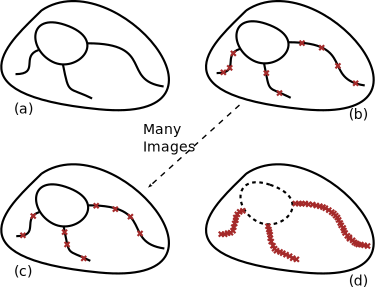
\includegraphics[width=0.8\linewidth]{STORM.pdf}
	\caption{STORM imaging. (a) The actual structure to be imaged is too small
	for regular microscopy. In stages (b) through (c), many images are taken,
	each with a different subset of the fluorescent markers activated. When
	the images are combined, (d), the points add up and reveal the nature
	of the object.}
	\label{fig:STORM}
\end{figure}
